\section{Model Refinement - Linear Drag Model}

Now that we are confident in our code architecture and we have proven that the simple parabolic model is inadequate, we can move on to developing the linear drag model. 

By linear drag we mean that, in addition to gravity, there is a new force which is linearly proportional to the projectile velocity and opposite in magnitude. 

\begin{align*}
\vec{F}_{\text{drag}} = -b\vec{v}
\end{align*}

With this drag force, and gravity, the equations of motions are derived by the video linked in the footnote.\footnote{Dr Ben Yelverton - Trajectory of a projectile with linear drag \href{https://www.youtube.com/watch?v=Tr\_TpLk3dY8}{https://www.youtube.com/watch?v=Tr\_TpLk3dY8}} We then used WolframAlpha to evaluate the derivatives for velocity and acceleration, and the final model is as follows:

% Linear Drag Model
\begin{align*}
&Model_{\text{Linear Drag}} = \\
&\begin{cases} 
\displaystyle \ddot{\bf r}(t) = \left[-\frac{1}{m}e^{-bt/m}(b\dot{\bf r}_{0y}+gm)\right]\hat{y} + \left[-\frac{b}{m}\dot{\bf r}_{0x}e^{-bt/m}\right]\hat{x} 
\\
\displaystyle \dot{\bf r}(t) = \left[\frac{1}{b}e^{-bt/m}(b\dot{\bf r}_{0y}+gm)-\frac{gm}{b}\right]\hat{y} + \left[\dot{\bf r}_{0x}e^{-bt/m}\right]\hat{x} 
\\
\displaystyle {\bf r}(t) = \left[\frac{m}{b}(\dot{\bf r}_{0y}+\frac{mg}{b})(1-e^{-bt/m})-\frac{mgt}{b}\right]\hat{y} + \left[\frac{m\dot{\bf r}_{0x}}{b}(1-e^{-bt/m})\right]\hat{x} + {\bf r}_0\\
t_{impact} = t > 0\text{ where }{\bf r}_y(t) = 0
\end{cases}
\end{align*}

where $g=9.81m/s^2$ is the acceleration due to gravity, ${\bf r}_0$ is the initial position, $\dot{\bf r}_0$ is the initial velocity, $\hat{y}$ is the unit vector in the upwards vertical direction, and $\hat{x}$ is the unit vector in the right direction. The projectile mass will be set to $m=1$ and $b$ will be fit by gradient descent.\footnote{We believe setting $m=1$ and fitting $b$ with gradient descent is valid if you're only interested in the projectile's trajectory and not the actual drag coefficient value.} A portion of the code implementation of this model is shown in Fig.~\ref{fig:model_matlab_code_lineardrag}.

\begin{figure}[t]
\centering
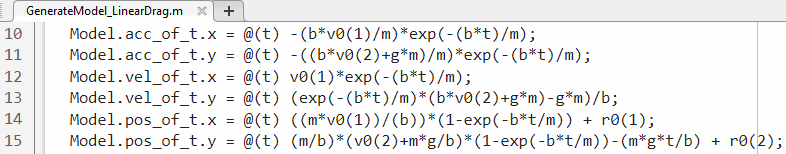
\includegraphics[width=\linewidth]{images/model_matlab_code_lineardrag.png}
\caption{\label{fig:model_matlab_code_lineardrag} Equations of motion for an object experiencing linear aerodynamic drag implemented in MATLAB. Full code available on GitHub.}
\end{figure}

Don't worry about fully understanding those equations too much. None of us did. Just because we know \LaTeX\ doesn't mean we're savants. What we're interested in is if it can form a trajectory that fits better than the parabolic model. If you're a frickin nerd and you \textit{do} want to analyze the math, take a look at the velocity function. Notice there's the exponential decay term of the form $e^{-t}$. For the $y$ component of the velocity, there will be some terminal velocity it reaches. For the $x$ component of velocity, it'll tend to 0. 

Thanks to our modular code architecture, we're able to implement this model as a new function file with no change to the rest of the code architecture. We can run our analysis with either version of the model by just changing an option value.
